\documentclass[12pt, titlepage]{article}

\usepackage{fullpage}
\usepackage[round]{natbib}
\usepackage{multirow}
\usepackage{booktabs}
\usepackage{tabularx}
\usepackage{float}
\usepackage{amsfonts}
\usepackage{graphicx}
\usepackage{float}
\usepackage{hyperref}
\hypersetup{
    colorlinks,
    citecolor=black,
    filecolor=black,
    linkcolor=red,
    urlcolor=blue
}
\usepackage[round]{natbib}

\newcounter{acnum}
\newcommand{\actheacnum}{AC\theacnum}
\newcommand{\acref}[1]{AC\ref{#1}}

\newcounter{ucnum}
\newcommand{\uctheucnum}{UC\theucnum}
\newcommand{\uref}[1]{UC\ref{#1}}

\newcounter{mnum}
\newcommand{\mthemnum}{M\themnum}
\newcommand{\mref}[1]{M\ref{#1}}

\title{SE 3XA3: Module Guide \\Poker Project}

\author{Team 12
        \\ Safwan Hossain and hossam18
        \\ Eamon Earl and earle2
        \\ Tyler Magarelli and magarelt
}

\date{April 12, 2022}

% \input{../../Comments}

\begin{document}

\maketitle

\pagenumbering{roman}
\tableofcontents
\listoftables
\listoffigures

\begin{table}[bp]
\caption{\bf Revision History}
\begin{tabularx}{\textwidth}{p{3cm}p{2cm}X}
\toprule {\bf Date} & {\bf Version} & {\bf Notes}\\
\midrule
March 16, 2022 & 1.0 & Initial Draft\\
March 18, 2022 & 1.1 & Revised Draft\\
April 12, 2022 & 2.0 & Revision 1\\
\bottomrule
\end{tabularx}
\end{table}

\newpage

\pagenumbering{arabic}

\section{Introduction}

\subsection{Summary of Project}

Our Poker Project is aptly named; we aim to build upon a relatively primitive base code for evaluating poker hand states and create a fully playable online poker experience. Our main motivation behind developing this software is to remove the barriers that other similar products have neglected to in the past, namely the requirement of financial commitment from the user. We firmly believe in the educational and developmental value of a strategic, high-stakes main.model.game like poker, but we also believe that losing money and promoting detrimental habits and addiction are not inherent to that high-stakes feeling. Our project will make this main.model.game accessible to students and other young people who are not in the financial situation to regularly go to a casino or use a monetary gambling app, and will give them the opportunity to develop valuable risk analysis skills and have fun with their friends, without the chance of harming their future.

\subsection{Context of Module Guide}

This document underlines the distinctions made using the information gathered from the requirements document, and how they will go on to partition the elements of the software into distinct modules, which are described in detail in the MIS below (Section 8). We have also developed traceability matrices to ensure that we have both encapsulated all of our required behaviour somewhere within the specification of the current architecture, and that our anticipated changes will have a "future home" as well. This document will provide various views on where we are currently at in the development process, where we were and where we intend on going, such that it will have some inherent value to each stakeholder involved. These include:

\begin{itemize}
    \item Designers: This document will act as an oracle for the design and dependencies of the programs to be written by the development team, showing both what is expected and likely areas of faults or stress, so that the designers can reinforce the importance of those areas and ensure that the developers are implementing them correctly. It also acts as information hiding, so when verifying the final product the design team can simply refer to the overarching hierarchy and behaviour described by the MIS, as opposed to reading through the code or its associated documentation. Additionally, as designing for generality is a specific property that we have prioritized given the possible application of the software to additional card main.model.game simulations, and we have already begun the process of considering anticipated changes, it allows the designers to freely consider what areas of the program may have the flexibility to accommodate for these heuristics.
    \item Developers: The viewpoint of this document that is most applicable to the developers is that of the MIS; the technical specification of what each module and their encapsulated routines must achieve. If the designers are vigilant and the requirements are fully and unambiguously specified, the developer should not have to consider anything else. Regardless, the abstraction of the architecture is there for their consideration, and interfacing directly with the source code may also give them unique insight into areas for achieving the previously discussed heuristics of generality and modifiability.
    \item Clients: The clients can use this document as a metric of the degree to which their business requirements are being met, specifically with Sections 4 and 6. They can also validate whether or not any anticipated changes conflict with any of their prior expectations, or if any unlikely changes highlight new behaviour that they may want to reconsider. However, it must be acknowledged that prioritizing a change after it has already been deemed unlikely may inherently cause some code overhaul and some setback in the lifetime of the development.  
\end{itemize}

\subsection{Design Principles}

As previously discussed, the main principles we are hoping to achieve with our design are generality and modifiability / designing for change. This is based off of the principle that the lifespan of our project is relatively small and consequently so is the scope, and as such there is very likely to be further development on this code in the future with the addition of further features and main.model.game modes, just as this project was based and developed on top of some previous source code; such is the nature and the beauty of open source projects. These principles encapsulate other ones, however, which can be seen throughout our design. Modularity is a principle that boils down parts of the functional source code into the smallest, distinct sections, which we have designed to have high internal coupling and low cohesion with other such modules. This allows for a module to be swapped out with another in the future, with minimal effects on the rest of the program. We also designed our program following the MVC (Model-main.view.View-Controller) architecture, which inherently partitions the program into three main sections, such that concerns can be separated when working in each distinct region. It also distinguishes areas of the code that are most important to different stakeholders and for different purposes. The data main.model will be used as a base for the current main.model.game mode and all future main.model.game modes, while the main.view is the most important section when considering the user. The controllers act as individual scripts for each main.model.game mode, and the main.server.Server works to trigger the controllers and link communication between multiple clients. All of these abstracted sections connect with the rest of the system minimally, ensuring that changes to the system can be made easily.

\subsection{Outline}

The rest of the document is organized as follows. Section
\ref{SecChange} lists the anticipated and unlikely changes of the software
requirements. Section \ref{SecMH} summarizes the module decomposition that
was constructed according to the likely changes. Section \ref{SecConnection}
specifies the connections between the software requirements and the
modules. Section \ref{SecMD} gives a detailed description of the
modules. Section \ref{SecTM} includes two traceability matrices. One checks
the completeness of the design against the requirements provided in the SRS. The
other shows the relation between anticipated changes and the modules. Section
\ref{SecUse} describes the use relation between modules.

\section{Anticipated and Unlikely Changes} \label{SecChange}

This section lists possible changes to the system. According to the likeliness
of the change, the possible changes are classified into two
categories. Anticipated changes are listed in Section \ref{SecAchange}, and
unlikely changes are listed in Section \ref{SecUchange}.

\subsection{Anticipated Changes} \label{SecAchange}

Anticipated changes are the source of the information that is to be hidden
inside the modules. Ideally, changing one of the anticipated changes will only
require changing the one module that hides the associated decision. The approach
adapted here is called design for
change.

\begin{description}
\item[\refstepcounter{acnum} \actheacnum \label{acHardware}:] Using a higher fidelity main.server.
\item[\refstepcounter{acnum} \actheacnum \label{acInput}:] Implementing the chip betting system with preset chip values (5, 10, 20, 100, etc.)
\item[\refstepcounter{acnum} \actheacnum \label{acData}:] The format of the data that is exchanged between the clients and the main.server.
\item[\refstepcounter{acnum} \actheacnum \label{acSync}:] The method of how all clients synchronize gameplay.
\item[\refstepcounter{acnum} \actheacnum \label{acSync}:] The addition of a main.controller template, that all main.controller classes will implement, to make running various main.model.game modes from the same starting menu easier.
\item[\refstepcounter{acnum} \actheacnum \label{acSync}:] main.view.GameView will be developed to have more useful display functionality, to relieve some complication of scripting gameplay in the main.controller, improving readability and fixing some cohesion issues.
\end{description}

\subsection{Unlikely Changes} \label{SecUchange}

%DELETE
The module design should be as general as possible. However, a general system is
more complex. Sometimes this complexity is not necessary. Fixing some design
decisions at the system architecture stage can simplify the software design. If
these decision should later need to be changed, then many parts of the design
will potentially need to be modified. Hence, it is not intended that these
decisions will be changed.

\begin{description}
\item[\refstepcounter{ucnum} \uctheucnum \label{ucIO}:] Input/Output devices (Input: File and/or Keyboard, Output: File, Memory, and/or Screen).
\item[\refstepcounter{ucnum} \uctheucnum \label{ucInput}:] There will always be a source of input data external to the software.
\item[\refstepcounter{ucnum} \uctheucnum:] A main.server will always be used for every main.model.game.
\item[\refstepcounter{ucnum} \uctheucnum:] The main.model for the deck will not change.
\end{description}

\section{Module Hierarchy} \label{SecMH}

This section provides an overview of the module design. Modules are summarized
in a hierarchy decomposed by secrets in Table \ref{TblMH}. The modules listed
below, which are leaves in the hierarchy tree, are the modules that will
actually be implemented.

\begin{description}
\item [\refstepcounter{mnum} \mthemnum \label{mHH}:] Hardware-Hiding Module
\item [\refstepcounter{mnum} \mthemnum \label{mModel}:] Model Module
\item [\refstepcounter{mnum} \mthemnum \label{mView}:] main.view.View Module
\item [\refstepcounter{mnum} \mthemnum \label{mController}:] Controller Module
\end{description}


\begin{table}[H]
\centering
\begin{tabular}{p{0.3\textwidth} p{0.6\textwidth} }
\toprule
\textbf{Level 1} & \textbf{Level 2}\\
\midrule

{Hardware-Hiding Module} & ~ \\
\midrule

\multirow{12}{0.3\textwidth}{Model Module} 
& main.model.client.Client\\
& main.model.update.GameInfo\\
& main.server.Server\\
& main.model.game.Game\\
& main.model.player.Card\\
& main.model.player.Player\\
& main.util.HandEvaluator\\
& main.model.player.Deck\\
& main.enumeration.main.model.game.PlayerAction\\
\midrule

\multirow{2}{0.3\textwidth}{main.view.View Module}
& main.view.MainMenuView\\
& main.view.GameView\\
\midrule 

\multirow{3}{0.3\textwidth}{Controller Module} 
& main.controller.MainController\\
& main.controller.ClientControllerOld\\
& main.server.ClientHandler\\
\bottomrule

\end{tabular}
\caption{Module Hierarchy}
\label{TblMH}
\end{table}

\section{Connection Between Requirements and Design} \label{SecConnection}


The design for this system is intended to meet all the requirements established in the first SRS document. The system is broken down into modules that will have their own requirements and when the modules are put together, the system will satisfy all of the requirements. Table 1 shows the relationship between needs and modules. \ref{TblRT}.

\section{Module Decomposition} \label{SecMD}

Modules are decomposed according to the principle of ``information hiding''
proposed by \citet{ParnasEtAl1984}. The \emph{Secrets} field in a module
decomposition is a brief statement of the design decision hidden by the
module. The \emph{main.util.Services} field specifies \emph{what} the module will do
without documenting \emph{how} to do it. For each module, a suggestion for the
implementing software is given under the \emph{Implemented By} title. If the
entry is \emph{OS}, this means that the module is provided by the operating
system or by standard programming language libraries.  Also indicate if the
module will be implemented specifically for the software.

Only the leaf modules in the
hierarchy have to be implemented. If a dash (\emph{--}) is shown, this means
that the module is not a leaf and will not have to be implemented. Whether or
not this module is implemented depends on the programming language
selected.

% ========== HARDWARE ========== %
\subsection{Hardware Hiding Modules (\mref{mHH})}

\begin{description}
\item[Secrets:]The data structure and algorithm used to implement the virtual
  hardware.
\item[main.util.Services:]Serves as a virtual hardware used by the rest of the
  system. This module provides the interface between the hardware and the
  software. So, the system can use it to display outputs or to accept inputs.
\item[Implemented By:] OS
\end{description}

% ========== MODEL ========== %

\subsection{Model Module}
    \begin{description}
    \item[Secrets:] Decides how elements of main.model.game data will stored and updated.
    \item[main.util.Services:] This module will determine the structure of majority of the system. It will consist of all the data elements that will need to be stored in order to run the program and modules that will implement functions that determine how the data can be updated.
    \item[Implemented By:] --
    \end{description}

\subsubsection{ main.model.client.Client Module (\mref{mModel})}
    \begin{description}
    \item[Secrets:] The information and components for a user to interact with the main.server.
    \item[main.util.Services:] Stores information about the user that is needed by the main.server to identify and manipulate each unique client.
    \item[Implemented By:] main.controller.ClientControllerOld
    \end{description}

\subsubsection{ main.model.update.GameInfo Module (\mref{mModel})}
    \begin{description}
    \item[Secrets:] Decides how to store main.model.game data.
    \item[main.util.Services:] Stores important main.model.game data that will be communicated between a main.server and client.
    \item[Implemented By:] main.model.client.Client, main.controller.ClientControllerOld, main.server.ClientHandler
    \end{description}

\subsubsection{ main.server.Server Module (\mref{mModel})}
    \begin{description}
    \item[Secrets:] Decides how to store and manage client and main.server data.
    \item[main.util.Services:] Stores main.server and client data, allowing users to establish a connection to the main.server.
    \item[Implemented By:] main.controller.MainController
    \end{description}

\subsubsection{ main.model.game.Game Module (\mref{mModel})}
    \begin{description}
    \item[Secrets:] Decides to store important elements of the main.model.game.
    \item[main.util.Services:] Provides a system to store and manage elements of the main.model.game that will keep track of the main.model.game's progress.
    \item[Implemented By:] main.controller.ClientControllerOld
    \end{description}

\subsubsection{ main.model.player.Card Module (\mref{mModel})}
    \begin{description}
    \item[Secrets:] Stores information about a card.
    \item[main.util.Services:] Provides a way to store a card suite and rank in a single data type.
    \item[Implemented By:] main.model.game.Game, main.model.player.Deck
    \end{description}

\subsubsection{ main.model.player.Player Module (\mref{mModel})}
    \begin{description}
    \item[Secrets:] Stores information about a player.
    \item[main.util.Services:] Provides a way to store and represent each player of the main.model.game.
    \item[Implemented By:] main.model.game.Game
    \end{description}

\subsubsection{ main.util.HandEvaluator Module (\mref{mModel})}
    \begin{description}
    \item[Secrets:] Decides the card rankings of each player's hand.
    \item[main.util.Services:] Provides a way to assign each player a hand ranking for comparison.
    \item[Implemented By:] main.model.game.Game
    \end{description}

\subsubsection{ main.model.player.Deck Module (\mref{mModel})}
    \begin{description}
    \item[Secrets:] Stores information about a deck of cards
    \item[main.util.Services:] Provides functions and storage for a collection of cards.
    \item[Implemented By:] main.model.game.Game
    \end{description}
    
\subsubsection{ main.enumeration.main.model.game.PlayerAction Module (\mref{mModel})}
    \begin{description}
    \item[Secrets:] Stores information about valid main.model.game moves.
    \item[main.util.Services:] Provides a way to validate user inputs by confirming if their input is a valid main.model.game move.
    \item[Implemented By:] main.model.game.Game, main.model.update.GameInfo, main.server.ClientHandler, main.model.client.Client
    \end{description}
% ========== VIEW ========== %

\subsection{main.view.View Module}
    \begin{description}
    \item[Secrets:] Decides how elements of main.model.game data will be displayed to the user.
    \item[main.util.Services:] This module will provide the visual aspect of the program, providing modules that will allow the data in the program to be displayed to the user in a meaningful way. Almost all elements of the main.view module will be easily modifiable with minimal collateral to other code.
    \item[Implemented By:] --
    \end{description}

\subsubsection{ main.view.MainMenuView Module (\mref{mView})}
    \begin{description}
    \item[Secrets:] Decides how the main menu of the program will be displayed.
    \item[main.util.Services:] Provides a way to display and navigate the main menu. Also contains error and success messages.
    \item[Implemented By:] main.controller.MainController
    \end{description}
    
\subsubsection{ main.view.GameView Module (\mref{mView})}
    \begin{description}
    \item[Secrets:] Decides how the main.model.game will be visually represented to the user.
    \item[main.util.Services:] Provides a way to display all the elements of the main.model.game to the user in a meaningful way. Also contains error and success messages.
    \item[Implemented By:] main.controller.ClientControllerOld
    \end{description}

% ========== CONTROLLER ========== %

\subsection{Controller Module}

\begin{description}
\item[Secrets:] Decides and handles the software decision making process. When and what data will be manipulated by user input.
\item[main.util.Services:] This module will act as a mediator between the main.view, main.model and the user. It will utilize the main.view and the main.model to display data to the user and take in user input and decide how the user input will manipulate the data.
\item[Implemented By:] --
\end{description}

\subsubsection{ main.controller.MainController Module (\mref{mController})}
    \begin{description}
    \item[Secrets:] Decides how to enter and setup the main.model.game.
    \item[main.util.Services:] Provides an interface to users on how to set up and join a main.model.game.
    \item[Implemented By:] Hardware-Hiding Module
    \end{description}

\subsubsection{ main.controller.ClientControllerOld Module (\mref{mController})}
    \begin{description}
    \item[Secrets:] Decides how the user can manipulate main.model.game data according to a central main.server consisting of multiple players.
    \item[main.util.Services:] Acts as the "brain" of the program by providing a synchronous way to play the main.model.game with other online players.
    \item[Implemented By:] Hardware-Hiding Module
    \end{description}

\subsubsection{ main.server.ClientHandler Module (\mref{mController})}
    \begin{description}
    \item[Secrets:] Decides how the main.server should respond to user input.
    \item[main.util.Services:] Provides a way for users to communicate with the main.server behind the scenes
    \item[Implemented By:] Hardware-Hiding Module
    \end{description}

% ======== PART 6 ======== %


\section{Traceability Matrix} \label{SecTM}

This section shows two traceability matrices: between the modules and the
requirements and between the modules and the anticipated changes.

% the table should use mref, the requirements should be named, use something
% like fref
\begin{table}[H]
\centering
\begin{tabular}{p{0.2\textwidth} p{0.6\textwidth}}
\toprule
\textbf{Func. Req.} & \textbf{Modules}\\
\midrule
FR1 & \mref{mModel}, \mref{mView}\\
FR2 & \mref{mModel}, \mref{mView}\\
FR3 & \mref{mModel}, \mref{mView}\\
FR4 & \mref{mModel}, \mref{mView}, \mref{mController}\\
FR5 & \mref{mModel}, \mref{mController}\\
FR6 & \mref{mModel}, \mref{mController}\\
FR7 & \mref{mModel}\\
FR8 & \mref{mModel}\\
FR9 & \mref{mModel}\\
FR10 & \mref{mModel}, \mref{mView}, \mref{mController}\\
FR11 & \mref{mModel}, \mref{mView}\\
FR12 & \mref{mModel}, \mref{mView}\\
FR13 &\mref{mModel}, \mref{mView}, \mref{mController}\\
FR14 & \mref{mModel}, \mref{mView}, \mref{mController}\\
FR15 & \mref{mModel}, \mref{mView}, \mref{mController}\\
FR16 & \mref{mModel}, \mref{mView}, \mref{mController}\\
FR17 & \mref{mModel}, \mref{mController}\\
FR18 & \mref{mModel}, \mref{mController}\\
FR19 & \mref{mController}\\
FR20 & \mref{mModel}, \mref{mView}, \mref{mController}\\
FR21 & \mref{mModel}, \mref{mView}, \mref{mController}\\
FR22 & \mref{mModel}, \mref{mView}, \mref{mController}\\
FR23 & \mref{mModel}, \mref{mView}\\
FR24 & \mref{mModel}, \mref{mView}\\
FR25 & \mref{mModel}, \mref{mView}, \mref{mController}\\
FR26 & \mref{mModel}, \mref{mView}, \mref{mController}\\
FR27 & \mref{mModel}, \mref{mView}, \mref{mController}\\
FR28 & \mref{mModel}, \mref{mController}\\
FR29 & \mref{mModel}, \mref{mController}\\
FR30 & \mref{mModel}, \mref{mController}\\
\bottomrule
\end{tabular}
\caption{Trace Between Functional Requirements and Modules}
\label{TblRT}
\end{table}

\begin{table}[H]
\centering
\begin{tabular}{p{0.2\textwidth} p{0.6\textwidth}}
\toprule
\textbf{Non-Func. Req.} & \textbf{Modules}\\
\midrule
NFR1 & \mref{mHH}, \mref{mView}\\
NFR2 & \mref{mHH}\\
NFR3 & \mref{mHH}\\
NFR4 & \mref{mHH}, \mref{mController}\\
NFR5 & \mref{mHH}\\
NFR6 & \mref{mModel}, \mref{mController}\\
NFR7 & \mref{mHH}\\
NFR8 & \mref{mHH}\\
NFR9 & \mref{mHH}\\
NFR10 & \mref{mHH}\\
NFR11 & \mref{mHH}\\
NFR12 & \mref{mHH}, \mref{mController}\\
NFR13 & \mref{mHH}, \mref{mController}\\
\bottomrule
\end{tabular}
\caption{Trace Between Non-Functional Requirements and Modules}
\label{TblRT}
\end{table}

\begin{table}[H]
\centering
\begin{tabular}{p{0.2\textwidth} p{0.6\textwidth}}
\toprule
\textbf{AC} & \textbf{Modules}\\
\midrule
AC1 & \mref{mHH}\\
AC2 & \mref{mModel}\\
AC3 & \mref{mHH}\\
AC4 & \mref{mHH}\\
AC5 & \mref{mController}\\
AC6 & \mref{mView}, \mref{mController}\\
\bottomrule
\end{tabular}
\caption{Trace Between Anticipated Changes and Modules}
\label{TblACT}
\end{table}

\section{Use Hierarchy Between Modules} \label{SecUse}

In this section, the uses hierarchy between modules is
provided. A uses relation between module A and module B is defined to be that module A is dependant of module B to function correctly. For example, if module A uses module B then the correct functioning of A depends upon the availability of a correct
implementation of B. Figure \ref{FigUH} illustrates the use relation between
the modules for this program. It can be seen that the graph is a directed acyclic graph. Each level of the hierarchy provides a testable and functional component of the system, and higher-level modules are effectively simpler since they rely on lower-level modules.

\begin{figure}[H]
\centering
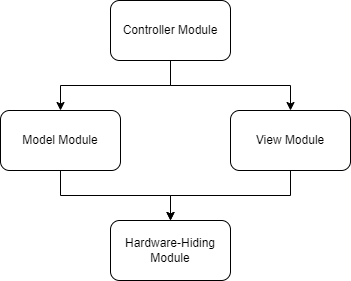
\includegraphics[width=0.7\textwidth]{Poker_UseDiagram.png}
\caption{Use hierarchy among modules}
\label{FigUH}
\end{figure}
\end{document}

